To compare the provisioning algorithms described above, we ran experiments
on two infrastructures: a homogeneous one (the DAS-4, a multi-cluster system
hosted by universities in The Netherlands~\cite{das4}) and a heterogeneous
one (the Amazon EC2 cloud~\cite{amazonEC2}). The goal of our experiments
was to compare the algorithms by how well they fulfill the SLOs and by
the amount of resources they allocate.

%In this section we conducted our experiments on a heterogeneous infrastructure like Amazon EC2~\cite{amazonEC2}, and on a homogeneous infrastructure like DAS-4 (the Distributed ASCI Supercomputer 4)~\cite{das4}. In our experiment campaign, we compared the degree of SLO enforcement and resource consumption for each provisioning algorithm implemented in ConPaaS. 

%DAS-4 is the Dutch Computational Infrastructure, a six-cluster wide-area distributed system designed with research purposes

\textbf{Testbed configuration:}  As a representative scenario, we deployed the MediaWiki application using ConPaaS on both infrastructures, and we ran the Wikibench tools with a 10\% sample of a real Wikipedia access trace for 24hours. 
%Consequently, our goal is to evaluate the behavior of the provisioning algorithms, when scaling out and back the number of VMs hosting PhP servers to guarantee several performance requirements, referred to as SLO.  Accordingly, some assumptions were made:
We configured the experiments as follows: 

\begin{itemize}
%\item  Response times from static requests were not analyzed due to its lightweight nature. 

\item The monitoring data was collected over a reporting period of 5 minutes.

\item We fixed a SLO of 700 milliseconds at the service's side (denoted by a red Line on Figures~\ref{naiveDas4},\ref{historyDas4},\ref{naiveEC2},\ref{historyEC2}).


\item The dynamic load-balancing weights provisioning technique was only evaluated on the heterogeneous platform, Amazon EC2. This algorithm brings improvements to the feedback algorithm only in environments where VMs may have different hardware configurations. 

\item The algorithms used the same statistically-chosen performance threshold ranges. 

%\item A minimum interval of 15 minutes has been established between scaling actions to avoid excessive oscillations. 
\end{itemize}


%To provide the Wikipedia services, an initial configuration was composed of 4 VMs, and 1 VM to host the Wikibench tools. The 4 VMs include a PhP service manager VM, a PhP agent VM, a web server and a http-proxy agent VM (both in the same VM), and finally a MySQL agent VM to store the English Wikipedia data, as explained in Section~\ref{wikipedia}.

\subsection*{Homogeneous Infrastructure}

Our experiments on DAS-4 rely on OpenNebula as IaaS~\cite{sotomayor_virtual_2009}. To deploy the Wikipedia services, we used small instances for the PHP service (manager and agents) and a medium instance for the MySQL service (agent). In DAS-4, OpenNebula's small instances provision VMs equipped with 1 CPU of 2Ghz, and 1GiB of memory, while medium instances are equipped with 4 CPU's of 2Ghz, and 4GiB of memory.

\paragraph{SLO enforcement.}
Figure~\ref{naiveDas4} and Figure~\ref{historyDas4} represent the degree of SLO fulfillment of the trigger-based and feedback algorithms, indicating the average of response times obtained during the execution of the Wikipedia workload trace. The results from Figure~\ref{naiveDas4} show that the trigger-based provisioning algorithm provokes an important amount of SLO violations at certain moments in time, due to its excessively reactive behavior. As we mentioned, this algorithm fails easily during traffic spikes, as adds or removes VMs without evaluating the workload trend. The feedback algorithm, as shown on Figure~\ref{historyDas4}, handles the traffic spikes better and can achieve fewer SLO violations; specifically, there were 31.72\% less SLO violations in comparison with the trigger-based algorithm. 


\begin{figure}

\begin{center}
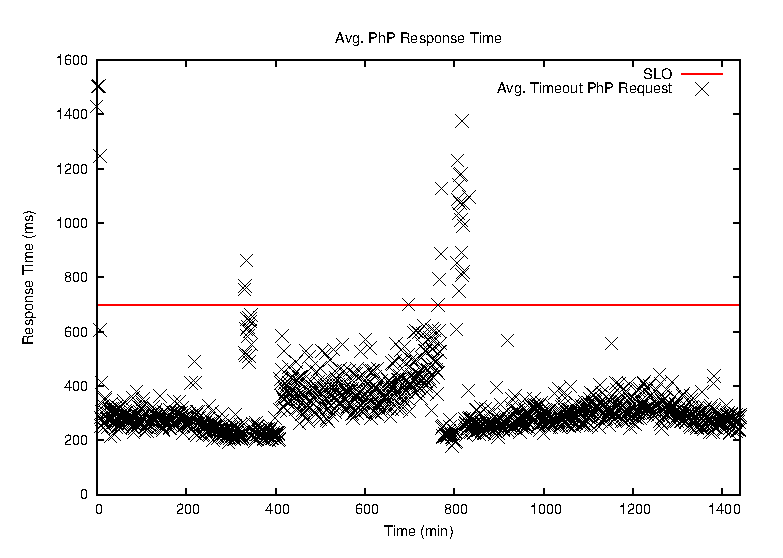
\includegraphics[width=0.49\textwidth, height=6cm]{./images/homogeneous/avgTimeout_PhP_trigger}
\end{center}
\vspace{-5mm}
\caption{Response time on DAS4 -- Trigger-based.}
\label{naiveDas4}
\end{figure}

\paragraph{Resource consumption.}

To better understand the behavior of both algorithms, we shall also focus on the resource consumption illustrated on Figure~\ref{resComDas4}. The excessively reactive behavior of the trigger-based algorithm can be noticed in the time intervals around \emph{t=350min} and \emph{t=820min}, where two scaling operations under-provision the system during a short period of time. These provisioning decisions provoked the SLO violations that are visible in Figure~\ref{naiveDas4}in the same intervals of time. Besides affecting the system's stability, such short fluctuations in the number of provisioned resource also raise the cost of hosting the application since more VM instantiations will be triggered. When using the feedback algorithm, the system makes provisioning decisions by analyzing workload's trend during a considerable interval of time. Scaling actions are only triggered when having \emph{constant} alterations in the workload, thereby providing a more efficient resource usage. Indeed, we can see that the provisioning decisions made by the feedback algorithm on Figure~\ref{resComDas4} match well with the workload alterations depicted on Figure~\ref{workload}.

\begin{figure}
\begin{center}
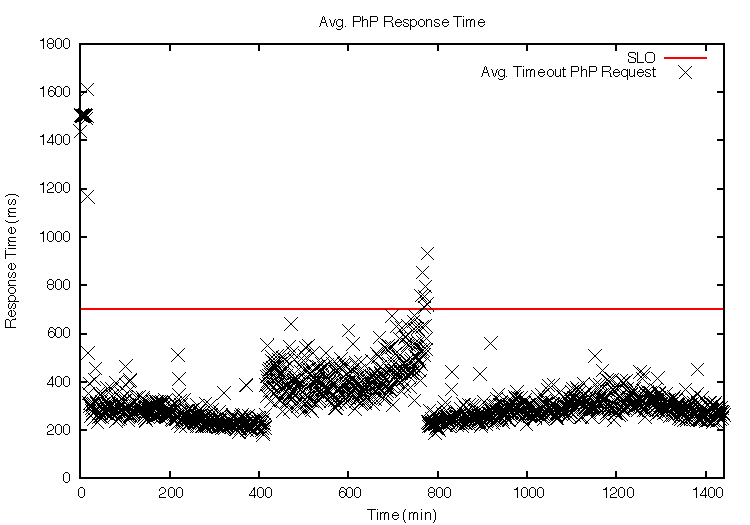
\includegraphics[width=0.49\textwidth, height=6cm]{./images/homogeneous/avgTimeout_PhP_feedback}
\end{center}
\vspace{-5mm}
\caption{Response time on DAS4 -- Feedback.}
\label{historyDas4}
\end{figure}

\begin{figure}
\begin{center}
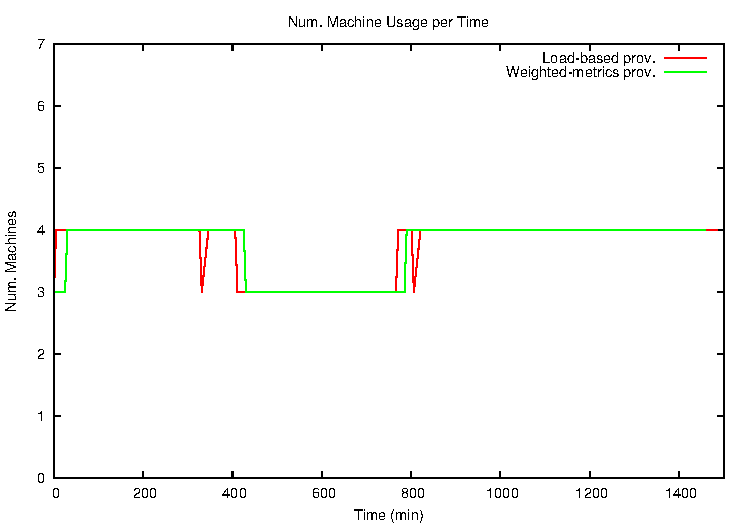
\includegraphics[width=0.49\textwidth, height=5cm]{./images/homogeneous/numMachinesComp}
\end{center}
\vspace{-5mm}
\caption{Resource consumption on DAS4.}
\label{resComDas4}
\end{figure}

\paragraph{Discussion.}

%Using the trigger-based provisioning algorithm, the system performance fluctuates greatly following a pattern similar to the web traffic, that increases the amount of SLO violations. The reactive behavior of this algorithm triggers scaling actions that affect to the system performance instead of improving it, and as a consequence, it is also wasteful in terms of resource consumption. Unlike feedback algorithm offers an efficient resource usage and a constant performance behavior while meeting the application's SLO. 

%Therefore this algorithm finds the trade-off between accuracy and cost savings.

%Both algorithms are best-effort regarding the SLO fulfillment, and thereby temporal alterations of the workload (with a short duration of 5min approx.) cannot be handled. The heterogeneity of the PhP-requests including images and requiring multiple Db queries, as well as the startup time of VMs (2-5min), are in part responsible of these SLO violations. 

Both algorithms are best-effort regarding the SLO fulfillment, and thus they do not handle well short alterations of the workload (with duration in the range of minutes). The heterogeneity of the PHP requests, as well as the startup time of VMs (2-5min), are in part responsible of these SLO violations.

%It avoid to under-provisioning in two occasions  while decreases the number of SLA violation. However, the naive alg. is vulnerable to temporal bursty workload variations (10 min), an increment of SLA violated is caused by under-provisioning operations in conjunction with workload variations. 



\subsection*{Heterogeneous Infrastructure}

Our experiments on EC2 used small instances for the PHP service (manager and agents) and  a medium instance for the MySQL service (agent). EC2 small instances provision VMs equipped with 1 EC2 CPU, and 1.7GiB of memory, while medium instances are equipped with 2 EC2 CPU's, and 3.75GiB of memory.

%In the following, we analyze the behavior of our algorithms when making provisioning decisions on a heterogeneous infrastructure.

\paragraph{SLO enforcement.}
Figure~\ref{naiveEC2}, Figure~\ref{historyEC2} and Figure~\ref{historyWeightEC2} show the system performance of the trigger-based, feedback and dynamic load-balancing weights algorithms, respectively. As depicted on Figure~\ref{naiveEC2}, the performance of the trigger-based algorithm is even more unstable than in the case of the homogeneous infrastructure. More precisely, two of the three peaks in response time, at \emph{t=300min} and \emph{t=820min}, can be explained by the variations in the Wikipedia workload shown in Figure~\ref{workload}. However, there is a third peak between \emph{t=400min} and \emph{t=500min} that corresponds to the interval of time on which the workload trace shows a significant drop in the request volumes. During this period of time, the algorithm attempts to scale down the system but since the smaller number of resources cannot handle the load, the system is scaled up again. As this algorithm does not keep any history information, it repeats this process of unsuccessful scaling, causing oscillations in the number of allocated resources.  

On the other hand, Figure~\ref{historyEC2} and Figure~\ref{historyWeightEC2} show as the feedback and dynamic load-balancing weight algorithm behave similarly. Even though both algorithms are best-effort, there is an important reduction in the number of SLO violations during the trace execution. In particular, the feedback algorithm reduces the SLO violations in a  41.3\%, while the dynamic load-balancing weights algorithm does it in a 47.6\%. Like on DAS-4, the feedback algorithm presents a stable performance pattern without having sudden and bursty workload alterations. Besides, as shown on Figure~\ref{historyWeightEC2}, the dynamic load-balancing weights algorithm algorithm has a similar behavior to the feedback algorithm in terms of system performance, however. This algorithm improves the SLO enforcement in a 6.3\% in comparison with feedback at the client's side. 

%Therefore we demonstrate how the use of workload-mix and flexible load-balancing techniques, although intrusive, do not cause time delays or excessive throughput alterations. 



\begin{figure}
\begin{center}
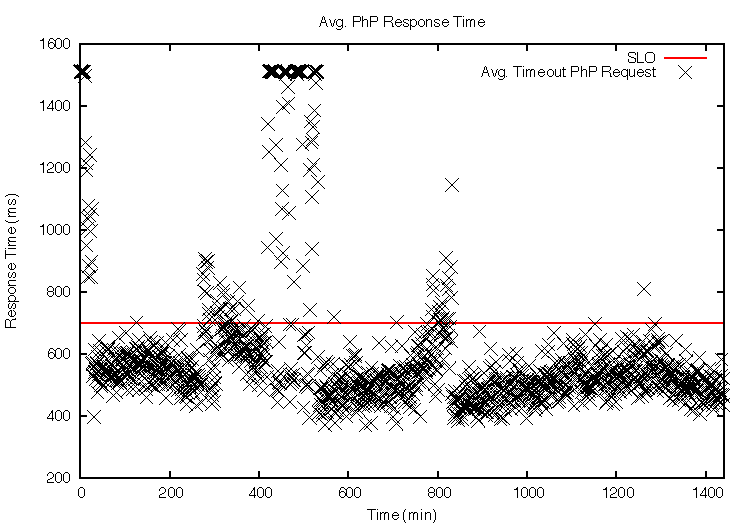
\includegraphics[width=0.49\textwidth, height=6cm]{./images/heterogeneous/avgTimeout_PhP_trigger}
\end{center}
\vspace{-5mm}
\caption{Response time on EC2 -- Trigger-based.}
\label{naiveEC2}
\end{figure}


\begin{figure}
\begin{center}
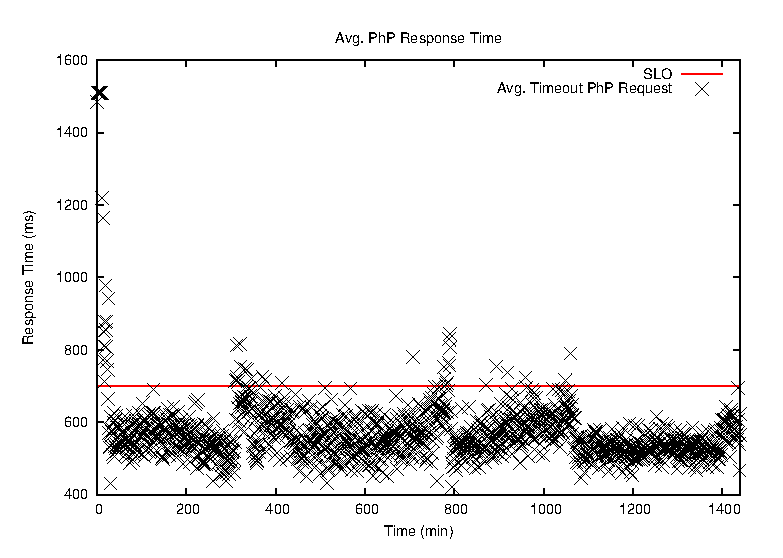
\includegraphics[width=0.49\textwidth, height=6cm]{./images/heterogeneous/avgTimeout_PhP_feedback}
\end{center}
\vspace{-5mm}
\caption{Response time on EC2-- Feedback.}
\label{historyEC2}
\end{figure}

\begin{figure}
\begin{center}
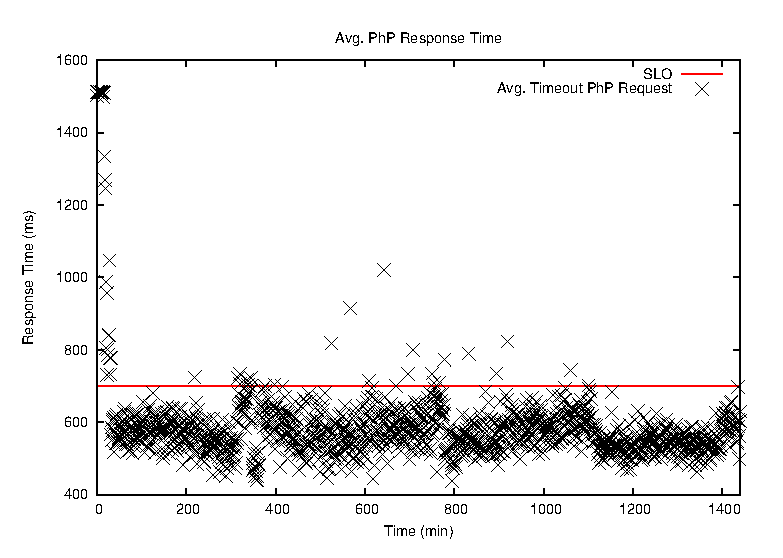
\includegraphics[width=0.49\textwidth, height=6cm]{./images/heterogeneous/avgTimeout_PhP_DLBweights}
\end{center}
\vspace{-5mm}
\caption{Response time on EC2-- Load-balancing Weights.}
\label{historyWeightEC2}
\end{figure}

\paragraph{Resource consumption.}

The resource usage on EC2 presents important changes, as shown on Figure~\ref{resEC2}. When using the trigger-based provisioning, the fluctuations in the system performance are explained as a result of a high frequency of scaling operations. In concrete, the fluctuations caused at the interval of time between \emph{t=400min} and \emph{t=500min} (see on Figure~\ref{naiveEC2}), match with the provisioning decisions made during the same interval of time on Figure~\ref{resEC2}. If we now pay attention to the feedback, and dynamic load-balancing weights algorithms, their resource consumptions are identical along the execution. Indeed, both algorithms decided to scale out the system during the interval of time comprised between \emph{t=1050min} and \emph{t=1400min}, to prevent future SLO violations that occurred when looking at the trigger-based algorithm on Figure~\ref{naiveEC2}. In particular, this situation demonstrates the benefits of using two-level threshold ranges to provide a predictive provisioning mechanism, thus improving the user experience.


\begin{figure}
\begin{center}
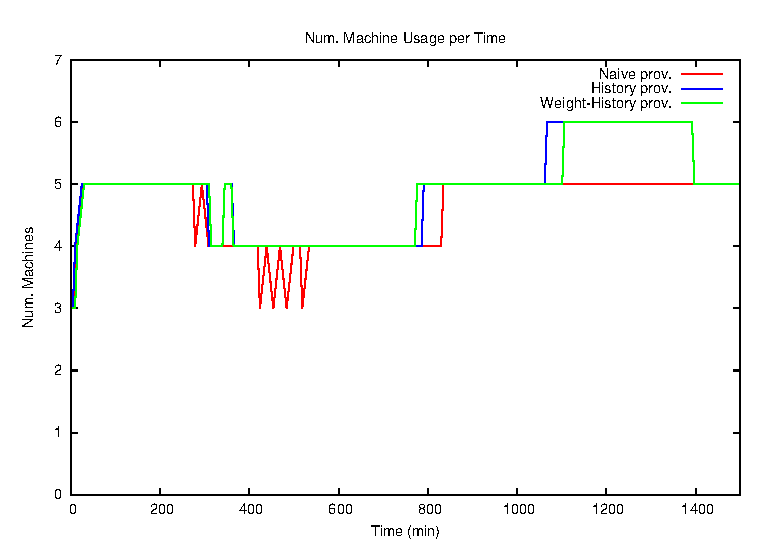
\includegraphics[width=0.49\textwidth, height=5cm]{./images/heterogeneous/numMachinesCompEC2}
\end{center}
\vspace{-5mm}
\caption{Resource consumption on EC2.}
\label{resEC2}
\end{figure}


\paragraph{Discussion.}
The experiments on EC2 leads to several conclusions. The use of the trigger-based algorithm shows again how aggressive provisioning increases the resource consumption and the chances of degraded application performance due to frequents scaling actions. These actions are triggered as an effect associated to the traffic and heterogeneity of the requests, when handling bursty workload conditions. On the other hand, the feedback and dynamic load-balancing algorithms constitute two robust provisioning models that offer an efficient resource consumption and keep stable the application performance during the trace execution. 

Furthermore, the use of a dynamic load-balancing algorithm provided a more efficient distribution of the request-mix across servers, that reduced the SLO violations in a 6.3\%. Hence, the main objective behind of this algorithm is to tackle the degradations caused by the workload heterogeneity.


%{\scriptsize
%\begin{table}
%\begin{center}
 %   \begin{tabular}{ | l | c | c |}
 %   \hline
 %  \textbf{Algorithm}   & \textbf{DAS4} & \textbf{EC2}   \\ \hline
 %   Load-based & 3808 &  30357    \\ \hline
 %   Feedback &	2601 & 17856 \\ \hline
 %   Dynamic load-balancing   & -- & 15931\\ \hline
%\textbf{Num. of requests}  & 384501 & 438430  \\ \hline
 %   \hline
	
  %  \end{tabular}
%\end{center}
%\caption{SLO violations at the client's side (1500ms).}
%\end{table}
%}


\subsection*{Discussion}



Generally, the result of our measurements show how the behavioral performance pattern and the resource consumption vary depending on the infrastructures on which we ran our experiments. Different hardware configurations such as those provided by DAS-4 and EC2, offer two distinct scenarios to validate our provisioning algorithms.  In these experiments, we demonstrate how trigger-based provisioning mechanisms can affect the system performance instead of improving it, as well as are wasteful in terms of resource usage. Furthermore, we show how a dynamic load-balancing technique, although intrusive, can be included and used without producing performance alterations. In fact, this technique slightly reduced the number of SLO violations in comparison with the results obtained using feedback algorithm. Finally, we also present the benefits by using feedback and dynamic load-balancing weights provisioning algorithms which aims to find the trade-off between the accuracy and cost savings. 

However, there is room for improvement using the dynamic load-balancing weights algorithm, as some  workload alterations could not be handled during the trace execution.

%the flexible threshold ranges were pre-defined before execution for all VMs. These threshold values might be %changed depending the type of instance to be provisioned. Therefore, we believe that offline profiling techniques %may be used to define these values depending of the type of instance, thus improving the effectiveness of our %predictions.

%Today's resource provisioning systems define SLO's based on desirable threshold values for an application (CPU %$<$ 70\% and resp. time $<$= 700ms). However, these threshold values change depending the type of instance %to be provisioned (\emph{i.e.,} small instances 200 $<$ resp. time $<$ 500, while medium instances 200 $<$ %response time $<$ 600). In order to improve the accuracy of these algorithms, we consider that provisioning %decisions have to take into account two threshold ranges: (i) desirable threshold values for the whole application; %(ii) specific threshold values for each machine. Thus, to determine these machine-specific threshold values, offline %profiling techniques have to train during a period of time 



